
\section{Fonctionalites}
\subsection{Description des fonctionalités}

         Notre projet à la possibilité de simuler le jeu de la vie, selon les règles de conway, du HighLife ou du Day \& Night. 
         \begin{figure}


 \begin{center}
    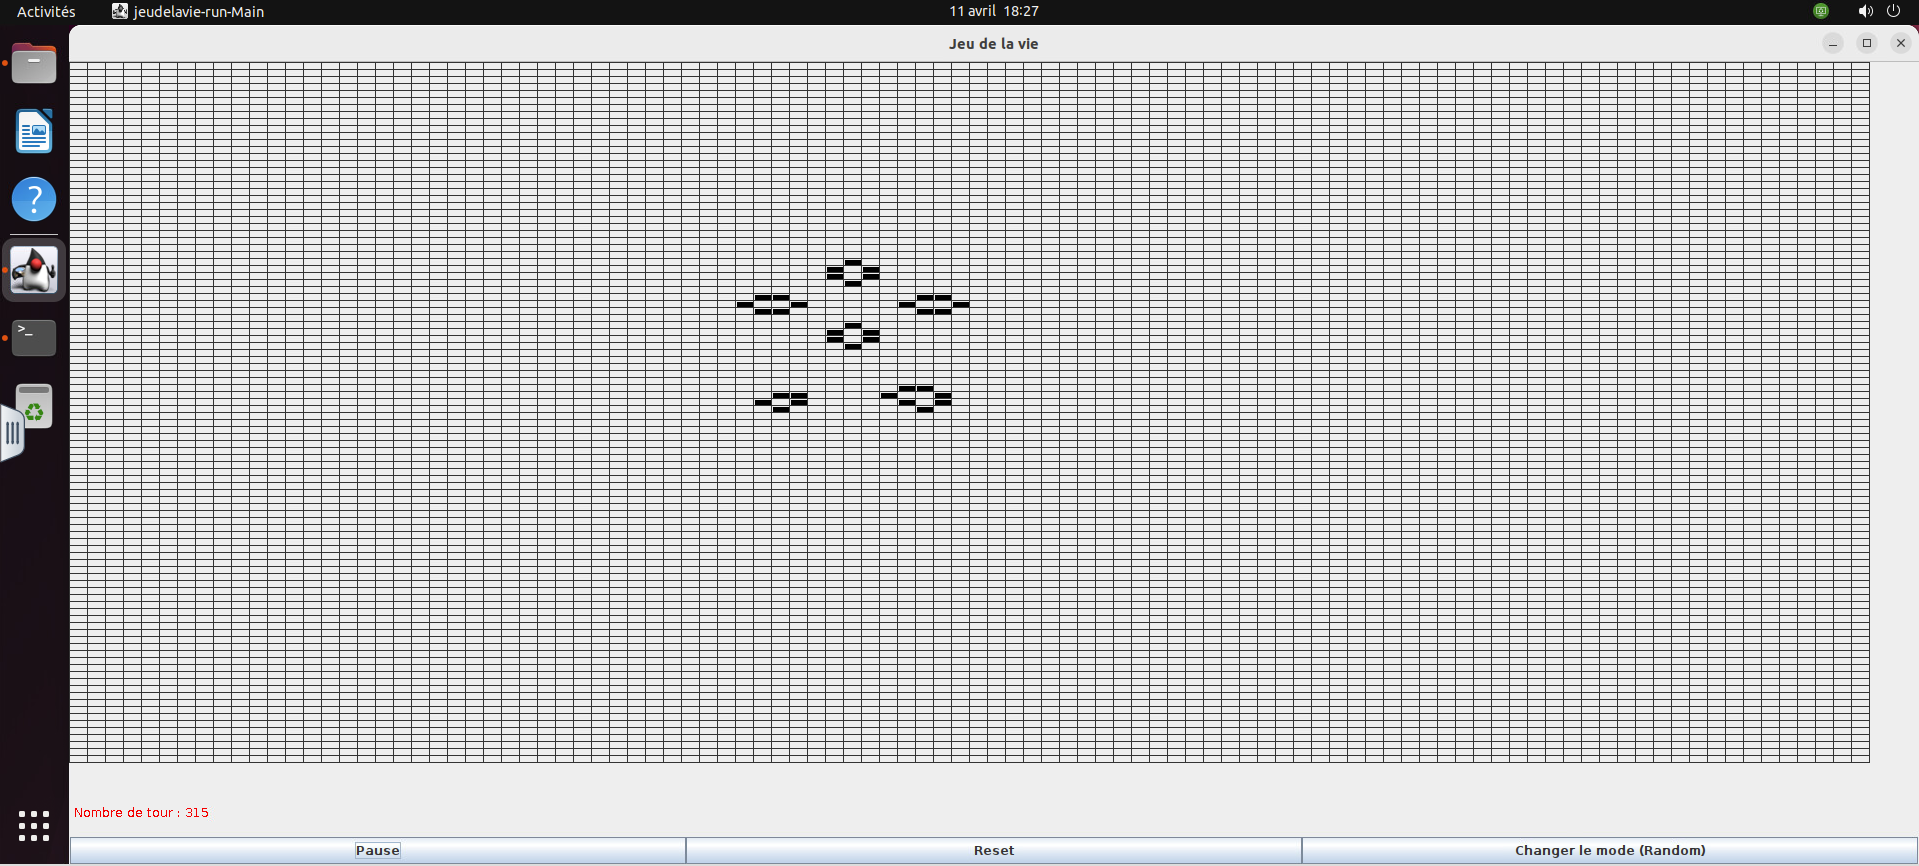
\includegraphics[width=120mm,scale=0.5]{figures/jeu.png}
    \captionof{figure}{Capture d'écran du jeu}
 \end{center}
         \end{figure}
    Avec comme cellules vivantes à la première génération, soit des cellules générés aléatoirement, importés depuis un fichier ou séléctionés sur la grille via des clicks sur l'interface graphique.
\begin{figure}
\begin{center}

    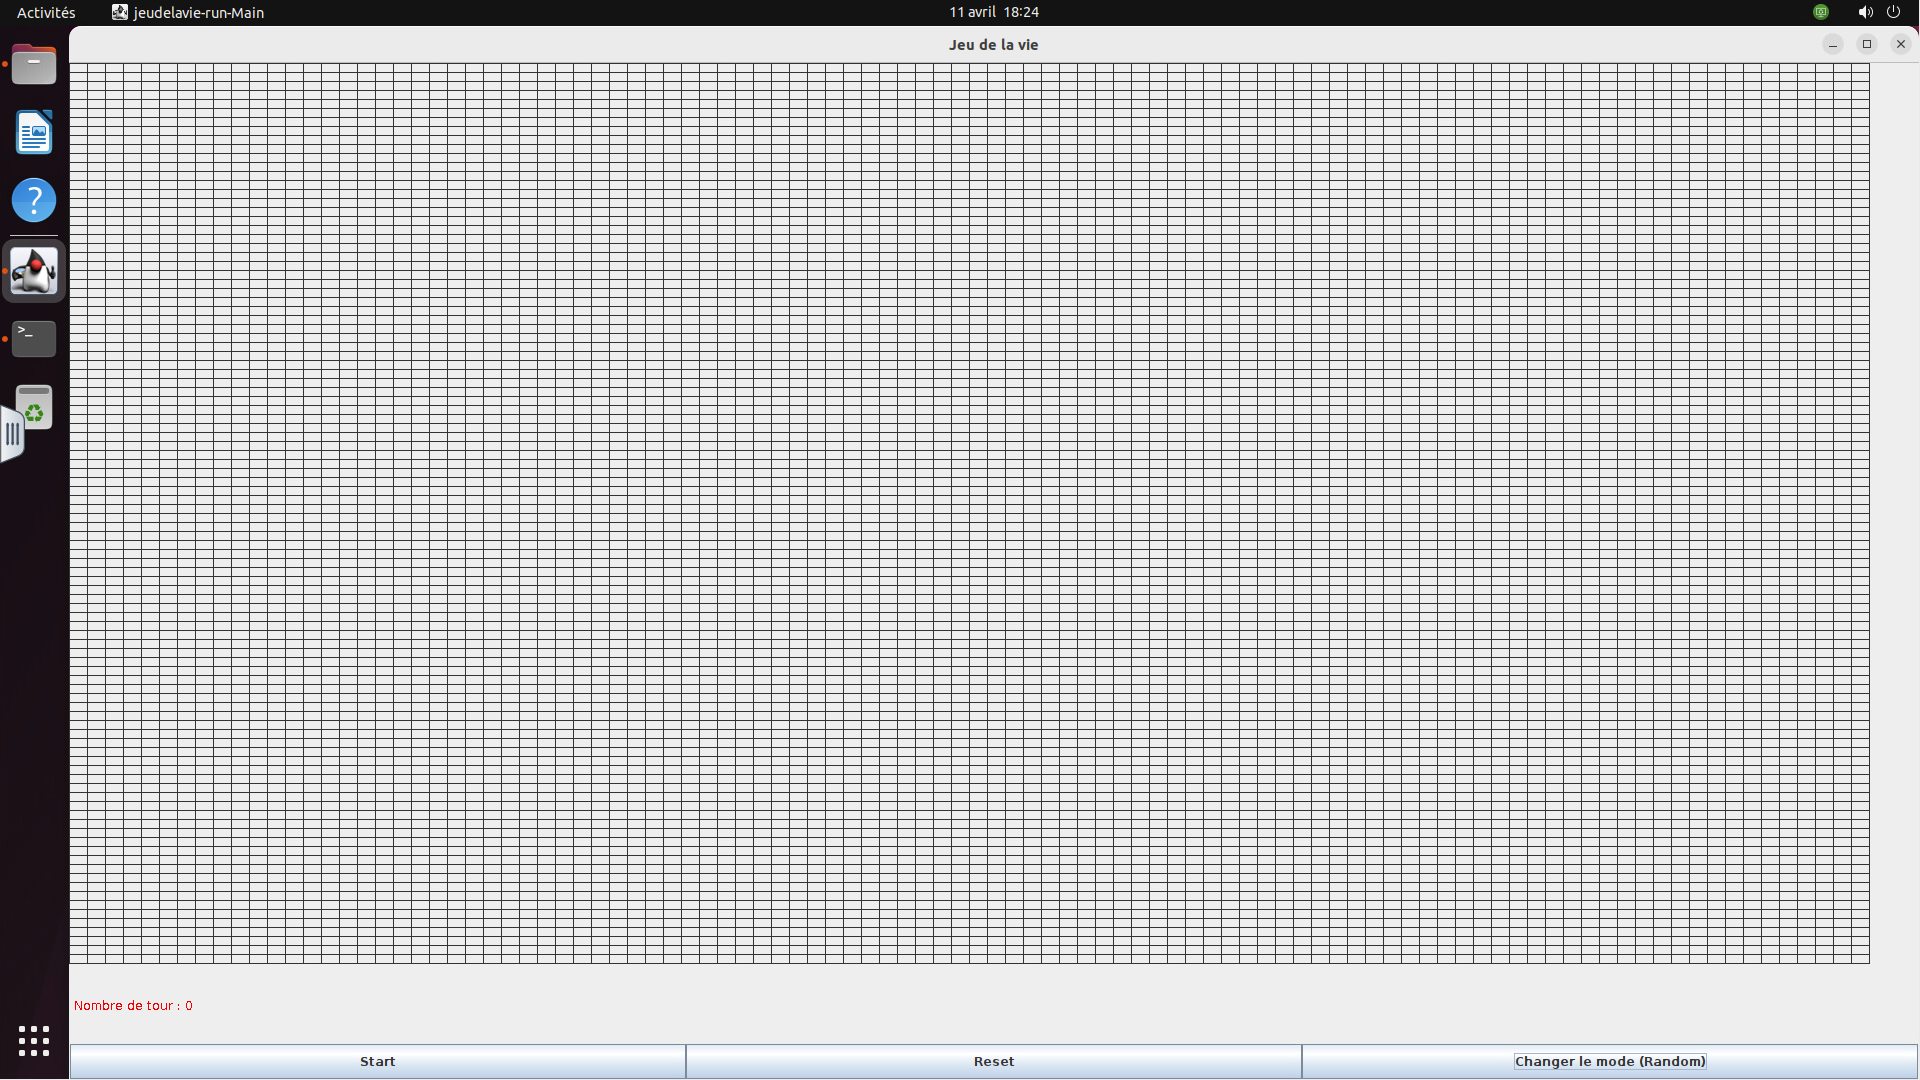
\includegraphics[width=120mm,scale=0.5]{figures/click_mode.png}
    \captionof{figure}{Mode grille cellules cliquables}

    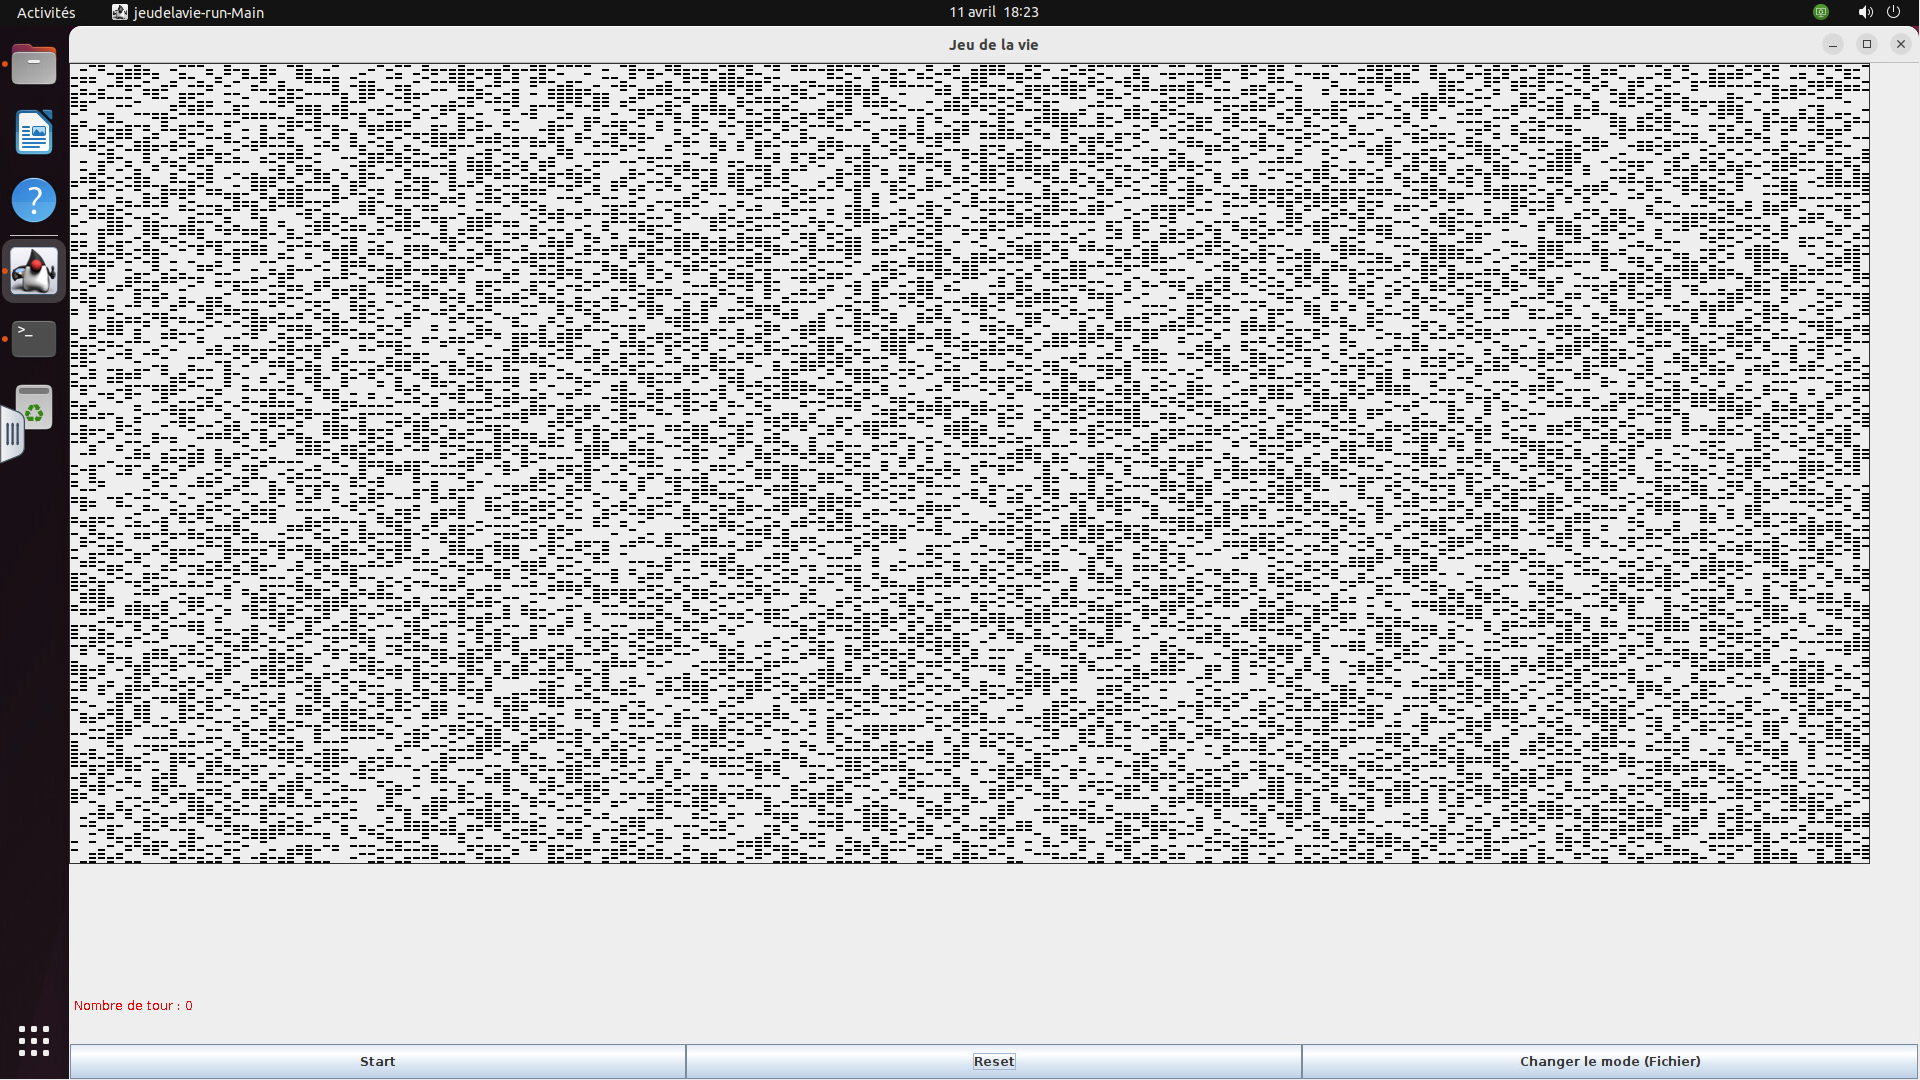
\includegraphics[width=120mm,scale=0.5]{figures/mode_random.png}
    \captionof{figure}{Génération de cellules aléatoirement sur la grille}
\end{center}
\end{figure}

    Le jeu est capable d'upscale comme de downscale, de switcher par exemple d'un affichage 100x100 à 10x10.
    \begin{figure}


\begin{center}
        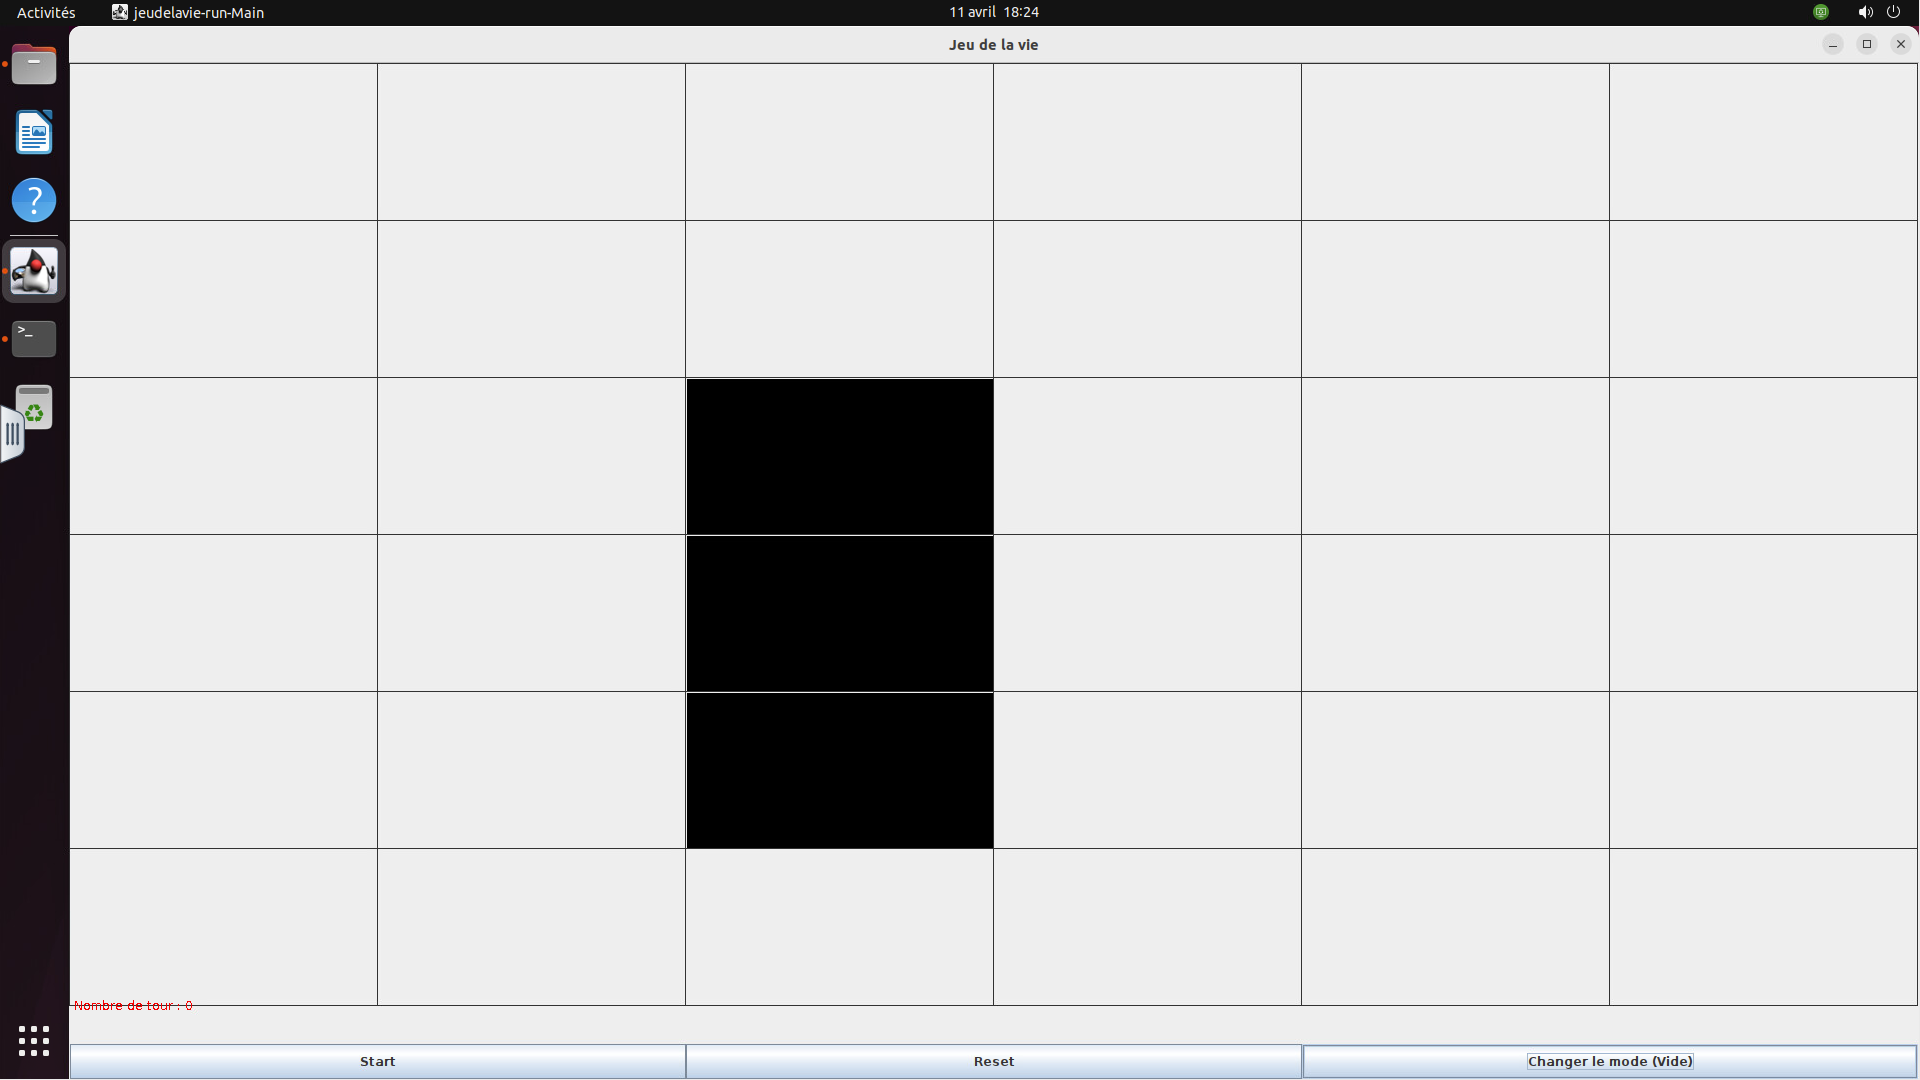
\includegraphics[width=120mm,scale=0.5]{figures/mode_file.png}
    \captionof{figure}{Mode grille depuis un fichier}
\end{center}
\end{figure}
    
    Avant le lancement de la simulation, sur l'interface graphique, 3 boutons sont visibles:

\begin{figure}

\begin{center}
    
\includegraphics[width=120mm,scale=0.5]{figures/start_btn.png}
    \captionof{figure}{Bouton "Start"}
    
    
\includegraphics[width=120mm,scale=0.5]{figures/pause_btn.png}
    \captionof{figure}{Bouton "Pause"}
    
    
\includegraphics[width=120mm,scale=0.5]{figures/reset_btn.png}
    \captionof{figure}{Bouton "Reset"}
    
    
\includegraphics[width=80mm,scale=0.5]{figures/change_btn.png}
    \captionof{figure}{Bouton "Changer de grille"}
\end{center}

\end{figure}

Pour lancer le jeu, il faut cliquer sur le bouton "Start", une fois que la simulation est lancée, le bouton devient "Pause" qui comme le nom l'indique, sert à mettre le jeu en pause.
Le bouton "Reset" permet de réinitialiser la grille et donc le compteur de génération. 
Le bouton "changer le mode" permet de switcher d'une façon de remplir la grille à une autre.

\begin{figure}
\begin{center}
    
\includegraphics[width=120mm,scale=0.5]{figures/compteur.png}
    \captionof{figure}{Compteur de générations}
\end{center}
    \end{figure}
    Avec ce compteur, il est possible de savoir à quelle génération le simulateur à évolué.
        \begin{figure}


\begin{center}
        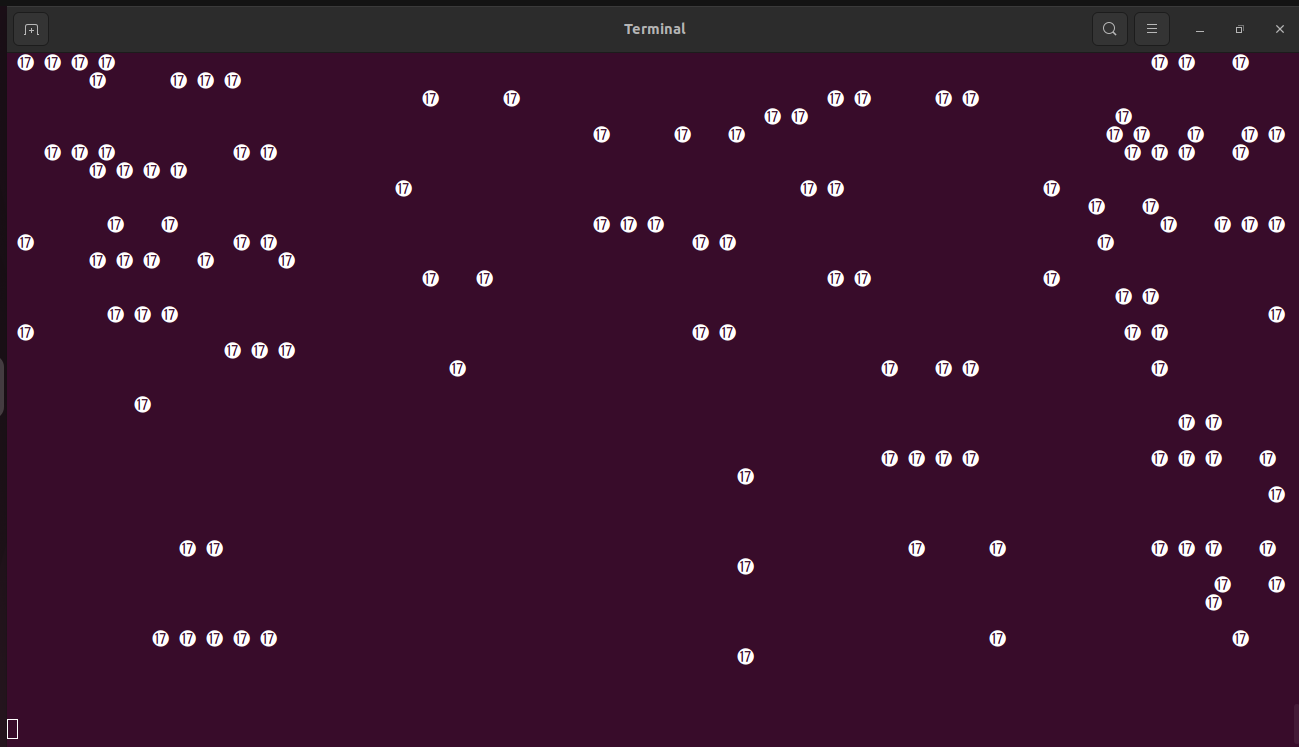
\includegraphics[width=120mm,scale=0.5]{figures/term.png}
    \captionof{figure}{Le jeu visible depuis le terminal}
\end{center}
\end{figure}


\subsection{Organisation du projet}

Dans un premier temps, la conception du logiciel à débuté avec une séance de brain-storming entre les membres du groupe sous la supervision du chargé de TP pour balancer les idées et propositions de chacun sur l'organisation du Projet

Différentes classes\ref{ref:les classes} :
Une fois d'accord sur les différentes classes nécessaires au développement du jeu, il était question de se repartir equitablement les tâches pour mener à bien le projet

Règles:
Certains membres du groupe étaient en charge de se renseigner sur les différents règles du jeu de la vie qui exsitent déjà et maîtiser les différences entre celles-ci.

Tests et Documentation :
L'intégration de tests unitaires pour assurer le bon fonctionnement des classes et des méthodes.

Pour la doc, la programmation par contrat nous a permis de générer automatiquement la Javadoc pour chaque classe et méthode du simulateur.

Outils collaboratifs :
Utilisation de GIT comme système de contrôle de version pour la modification des différents fichiers du simulateur.

Utilisation de Overleaf pour un suivi et accès du rapport et du PDF de la soutenance par toute l'équipe.
